\chapter{Implementación y Entorno de Desarrollo}\label{cap:implementacion}

\section{Introducción}
En este capítulo se describen las tecnologías utilizadas para la construcción de TraDeck, abarcando desde el entorno de pruebas de la capa de persistencia hasta el desarrollo de la interfaz de usuario.

\section{Entorno de Desarrollo: Hardhat vs. Remix}
Para el desarrollo y compilación de los Smart Contracts, la industria ofrece diversas alternativas, siendo \textit{Remix IDE} y \textit{Hardhat} las más destacadas. 

Aunque Remix proporciona una interfaz web excelente para pruebas rápidas y prototipado, se ha optado por \textbf{Hardhat} \cite{hardhat_docs} por los siguientes motivos arquitectónicos:

\begin{itemize}
	\item \textbf{Instancia Local de Base de Datos (Hardhat Network):} Hardhat levanta un nodo local de Ethereum que actúa como un servidor de base de datos aislado. Esto permite realizar pruebas destructivas, simular transacciones atómicas y evaluar el coste de operaciones (Gas) sin depender de redes externas ni incurrir en costes económicos.
	\item \textbf{Automatización y Testing:} A diferencia de Remix, Hardhat se integra de forma nativa en entornos Node.js, permitiendo programar \textit{scripts} de migración (despliegue de esquemas de datos) y tests unitarios automatizados para validar los cambios de estado en los contratos.
	\item \textbf{Gestión de Dependencias:} Facilita la importación de librerías como \textit{OpenZeppelin} mediante el gestor de paquetes NPM, manteniendo la infraestructura como código (IaC).
	\item \textbf{Usuarios de Prueba:} De forma nativa Hard Hat aporta 10 carteras, con dirección privada y pública y 1000 ETH de gas, cuentas que hemos usado en las pruebas locales.
\end{itemize}
\section{Conexión a la Base de Datos: Ethers.js}
En aplicaciones tradicionales, el backend utiliza diversos drivers para comunicarse con la base de datos. En TraDeck, esta función la cumple \textbf{Ethers.js} \cite{ethers_docs}. 

Esta librería actúa como el puente de comunicación entre nuestra interfaz frontend y el nodo de la blockchain de Ethereum. Permite inyectar el proveedor criptográfico del usuario (como MetaMask), firmar las transacciones de escritura (modificaciones de estado en los Smart Contracts) y realizar consultas de lectura gratuitas (como leer el balance de un usuario).

\section{Gestión de Identidad y Proveedor Inyectado: MetaMask}
A diferencia de los sistemas tradicionales que dependen de un servidor central para la autenticación (OAuth, JWT), TraDeck implementa un modelo de \textbf{identidad auto-soberana}. 

Se ha seleccionado \textbf{MetaMask} \cite{metamask_docs} como el proveedor inyectado (\textit{Injected Provider}) por ser el estándar de la industria. Técnicamente, su función en nuestra arquitectura es doble:
\begin{itemize}
	\item \textbf{Custodia de Claves Privadas:} MetaMask actúa como un almacén seguro de claves, evitando que la dApp tenga acceso directo a la clave privada del usuario, lo que garantiza la seguridad de los activos.
	\item \textbf{Gestión de Firmas:} Cada vez que el frontend solicita una operación de escritura en los Smart Contracts (ej. \texttt{listForSale}), MetaMask intercepta la petición, muestra al usuario los detalles y el coste de gas, y genera la firma criptográfica necesaria para que la red Ethereum valide la transacción.
\end{itemize}

\subsection{El concepto de Injected Provider}
Técnicamente, un \textit{Injected Provider} es un objeto JavaScript (estandarizado bajo la propuesta \textbf{EIP-1193} \cite{eip1193}) que las extensiones de billetera como MetaMask introducen en el espacio de nombres global del navegador (\texttt{window.ethereum}). 

Funciona, en esencia, como una capa de abstracción: permite que la dApp realice consultas y solicite firmas sin que los scripts de la página web tenga acceso directo a las claves privadas del usuario. Al no haber servidor backend tradicional es el frontend el encargado de hablar con la blockchain directamente, pero el frontend no puede (ni debe) guardar las claves privadas del usuario, ya que sería un agujero de seguridad brutal.


\section{Validación y Testing}
Para garantizar que nuestra base de datos distribuida se comporta correctamente ante fallos (por ejemplo, transacciones atómicas que deben revertirse), se han implementado tests unitarios en \textbf{Mocha} y \textbf{Chai}. Estas pruebas simulan múltiples usuarios (cuentas generadas por Hardhat) interactuando con el mercado, verificando que los estados del protocolo \textit{Escrow} se cumplen.

\section{Interfaz de Usuario}
La interfaz de TraDeck ha sido diseñada para mantener simplicidad, para evitar al usuario los problemas de lidiar directamente con una cadena de bloques.

\begin{figure}[H]
	\centering
	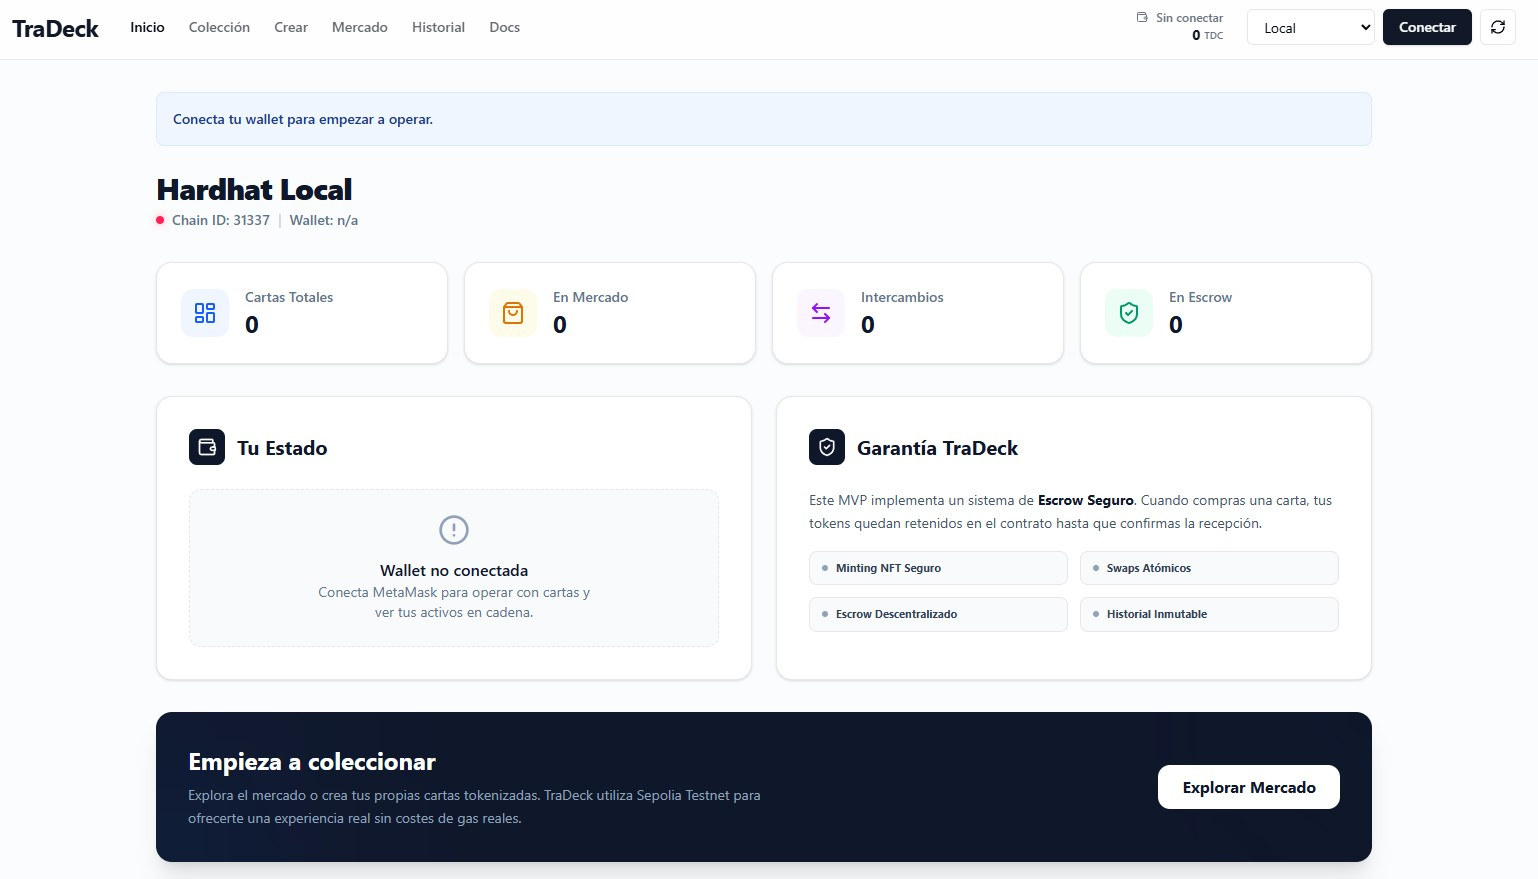
\includegraphics[width=0.8\textwidth]{img/index.jpg}
	\caption{Página de inicio de TraDeck: Punto de entrada y conexión con el proveedor inyectado.}
	\label{fig:index}
\end{figure}

\begin{figure}[H]
	\centering
	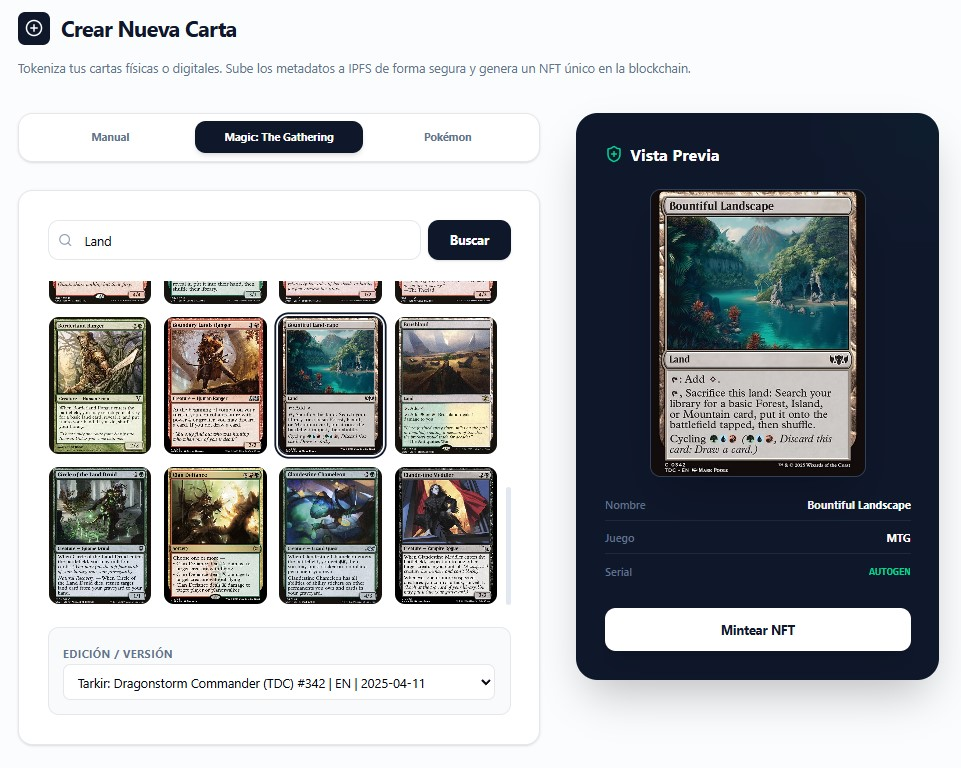
\includegraphics[width=0.8\textwidth]{img/crear.jpg}
	\caption{Módulo de Minting: Interfaz para la persistencia de nuevos activos en IPFS y Blockchain.}
	\label{fig:crear}
\end{figure}

\begin{figure}[H]
	\centering
	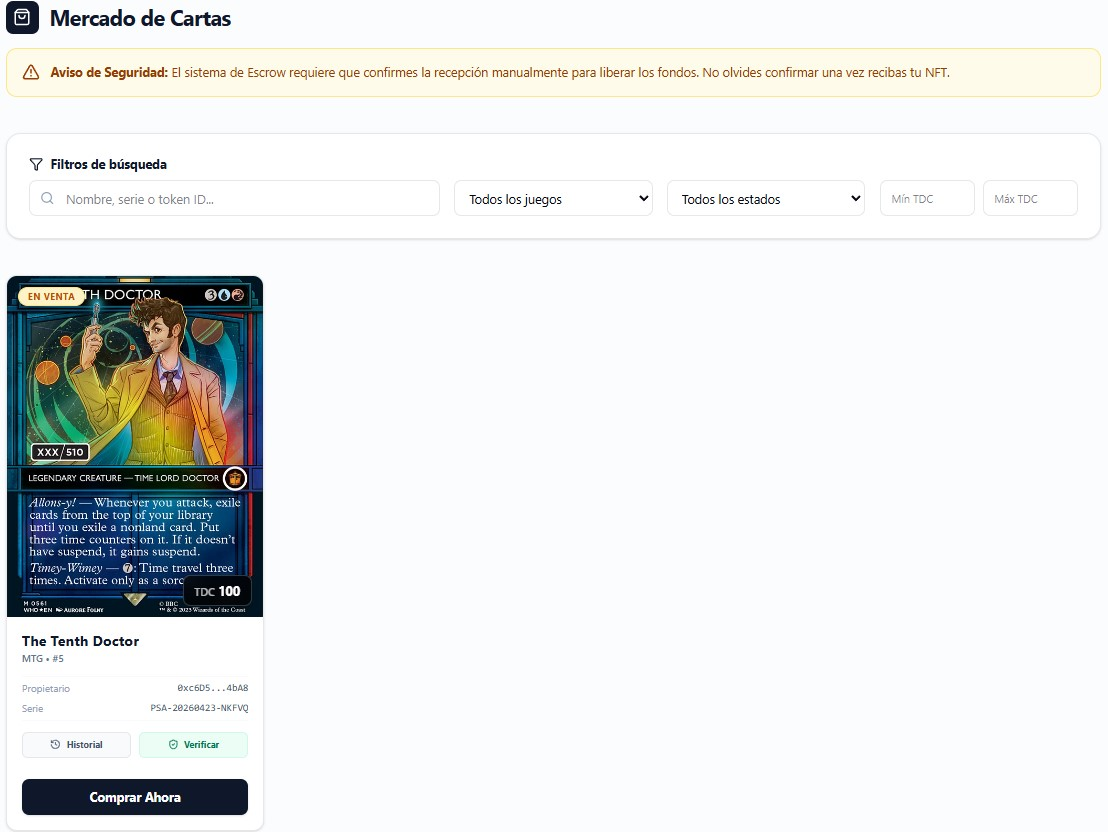
\includegraphics[width=0.8\textwidth]{img/mercado.jpg}
	\caption{Mercado Descentralizado: Visualización de ofertas activas en el Smart Contract.}
	\label{fig:mercado}
\end{figure}

\begin{figure}[H]
	\centering
	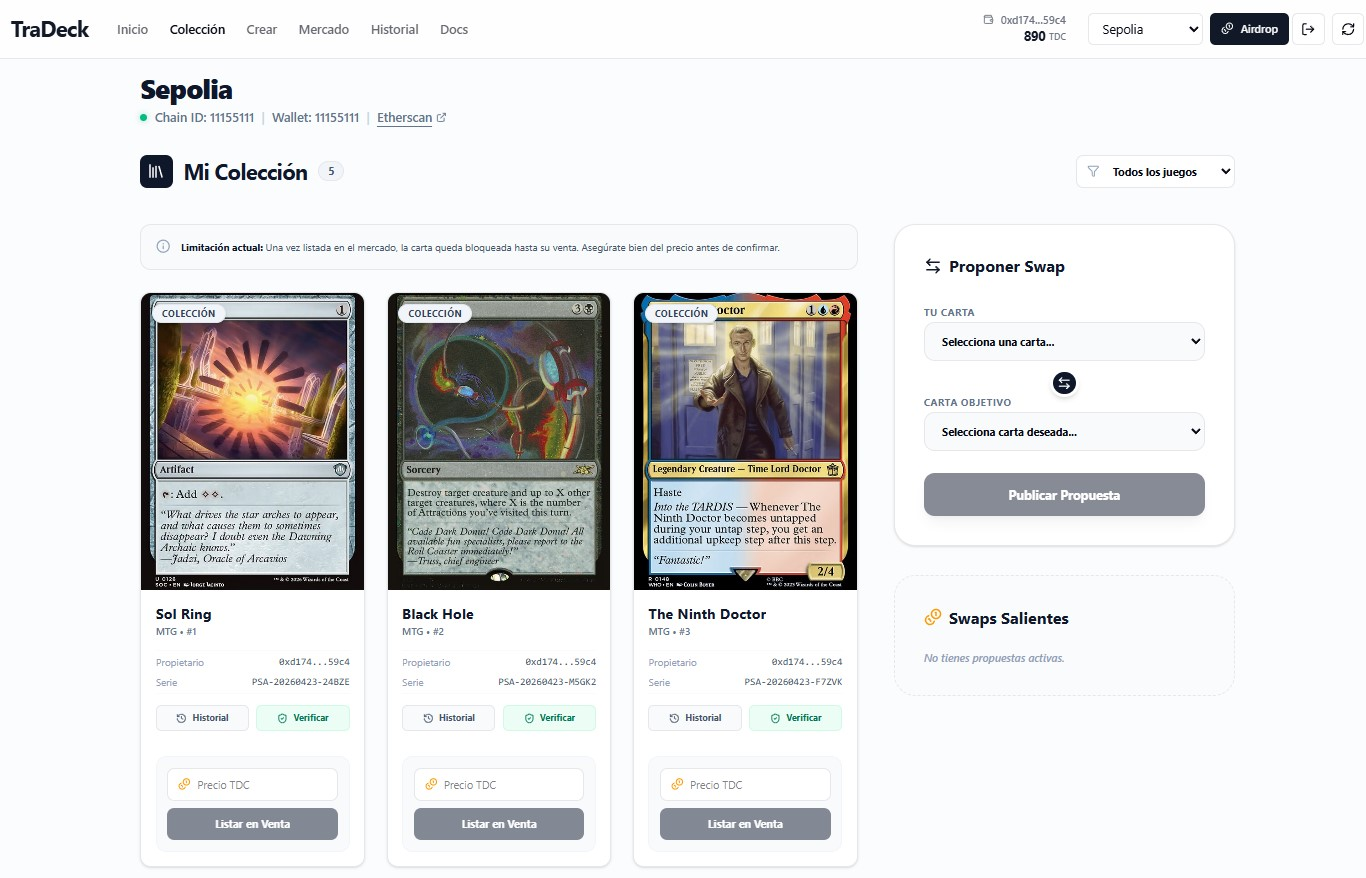
\includegraphics[width=0.8\textwidth]{img/micoleccion.jpg}
	\caption{Gestión de Inventario: Consulta en tiempo real de la propiedad de los tokens ERC-721.}
	\label{fig:coleccion}
\end{figure}

\begin{figure}[H]
	\centering
	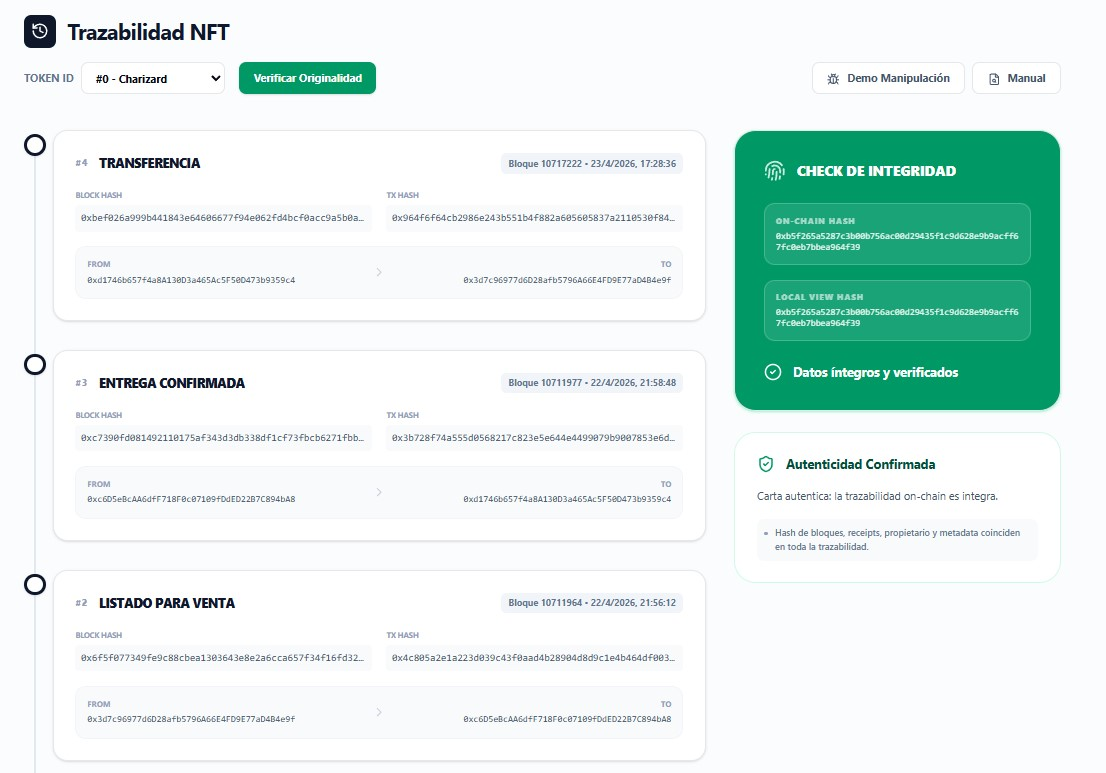
\includegraphics[width=0.8\textwidth]{img/trazabilidad.jpg}
	\caption{Historial de Trazabilidad: Registro inmutable de transacciones y cambios de estado del activo.}
	\label{fig:trazabilidad}
\end{figure}
